\chapter{Part II(b) - Processor, I/Os, and Exceptions W - 4.1 - 4.2}
\section{The CPU}

The CPU is a very sequential component responsible for executing instructions in a controlled manner. The CPU interacts with the memory through a defined memory interface, which includes various control signals and data pathways.
\begin{center}
    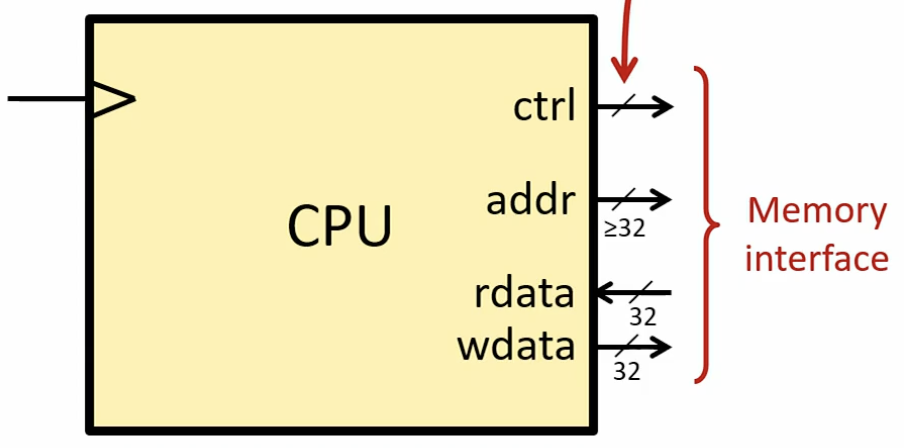
\includegraphics[width=0.45\textwidth]{chapters/chapter2b/images/cpu.png}
\end{center}
\begin{itemize}
    \item[-] \textbf{Control Signals (ctrl)}: These signals manage the behavior of memory access, indicating whether to read or write data.
    \item[-] \textbf{Address (addr)}: Specifies the memory address where the CPU wants to read or write data. The width of the address bus is typically 32 bits or more.
    \item[-] \textbf{Read Data (rdata)}: A 32-bit pathway through which the CPU receives data from the memory.
    \item[-] \textbf{Write Data (wdata)}: A 32-bit pathway through which the CPU sends data to be stored in memory.
\end{itemize}

The memory interface is also controlled by two important signals:
\begin{itemize}
    \item[-] \textbf{Circuit Enable (CE)}: Validates the address, indicating that the address provided is active and the operation should proceed.
    \item[-] \textbf{Write Enable (WE)}: Indicates that the current access is a store operation, allowing data to be written into memory.
\end{itemize}
\textbf{From now on, the clock signal, which drives the sequential behavior, may be omitted for simplicity.}
This interface design allows for a clear and structured method of communication between the CPU and memory, ensuring reliable execution of instructions and data management. \\
\begin{minipage}[htp]{0.45\textwidth}
    Some processors, instead of having two seperate buses, have a single data bus, that can be used for both reading and writing. This is known as a \texttt{bidirectional data bus}. This means, this kind of system uses a tri-state buffer to control the direction of the data flow.
\end{minipage}
\hfill
\vline
\hfill
\begin{minipage}[htp]{0.45\textwidth}
    \begin{center}
        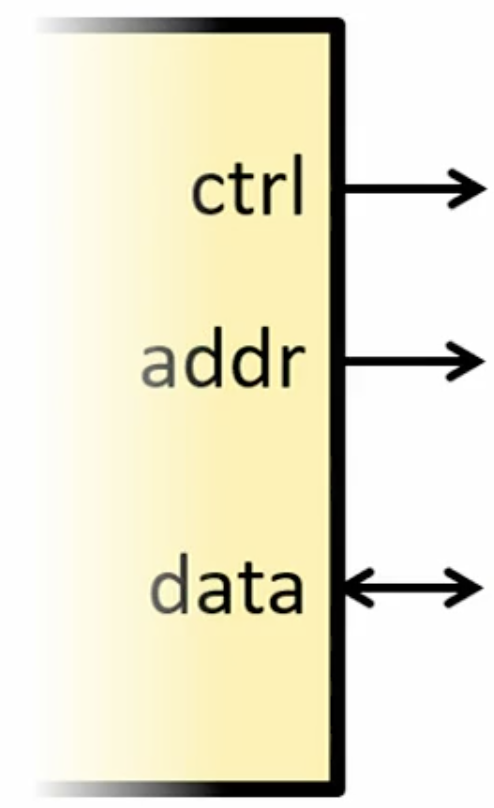
\includegraphics[width=0.35\textwidth]{chapters/chapter2b/images/tristate.png}
    \end{center}
\end{minipage}
\section{Physical Memory Map}
\textit{To connect the CPU to memory, we need to define a \texttt{physical memory map.} As we had 32 bits of address, we can address $2^{32}$ bytes of memory (aprox. 4GB of memory at least in a CPU).}
\begin{center}
    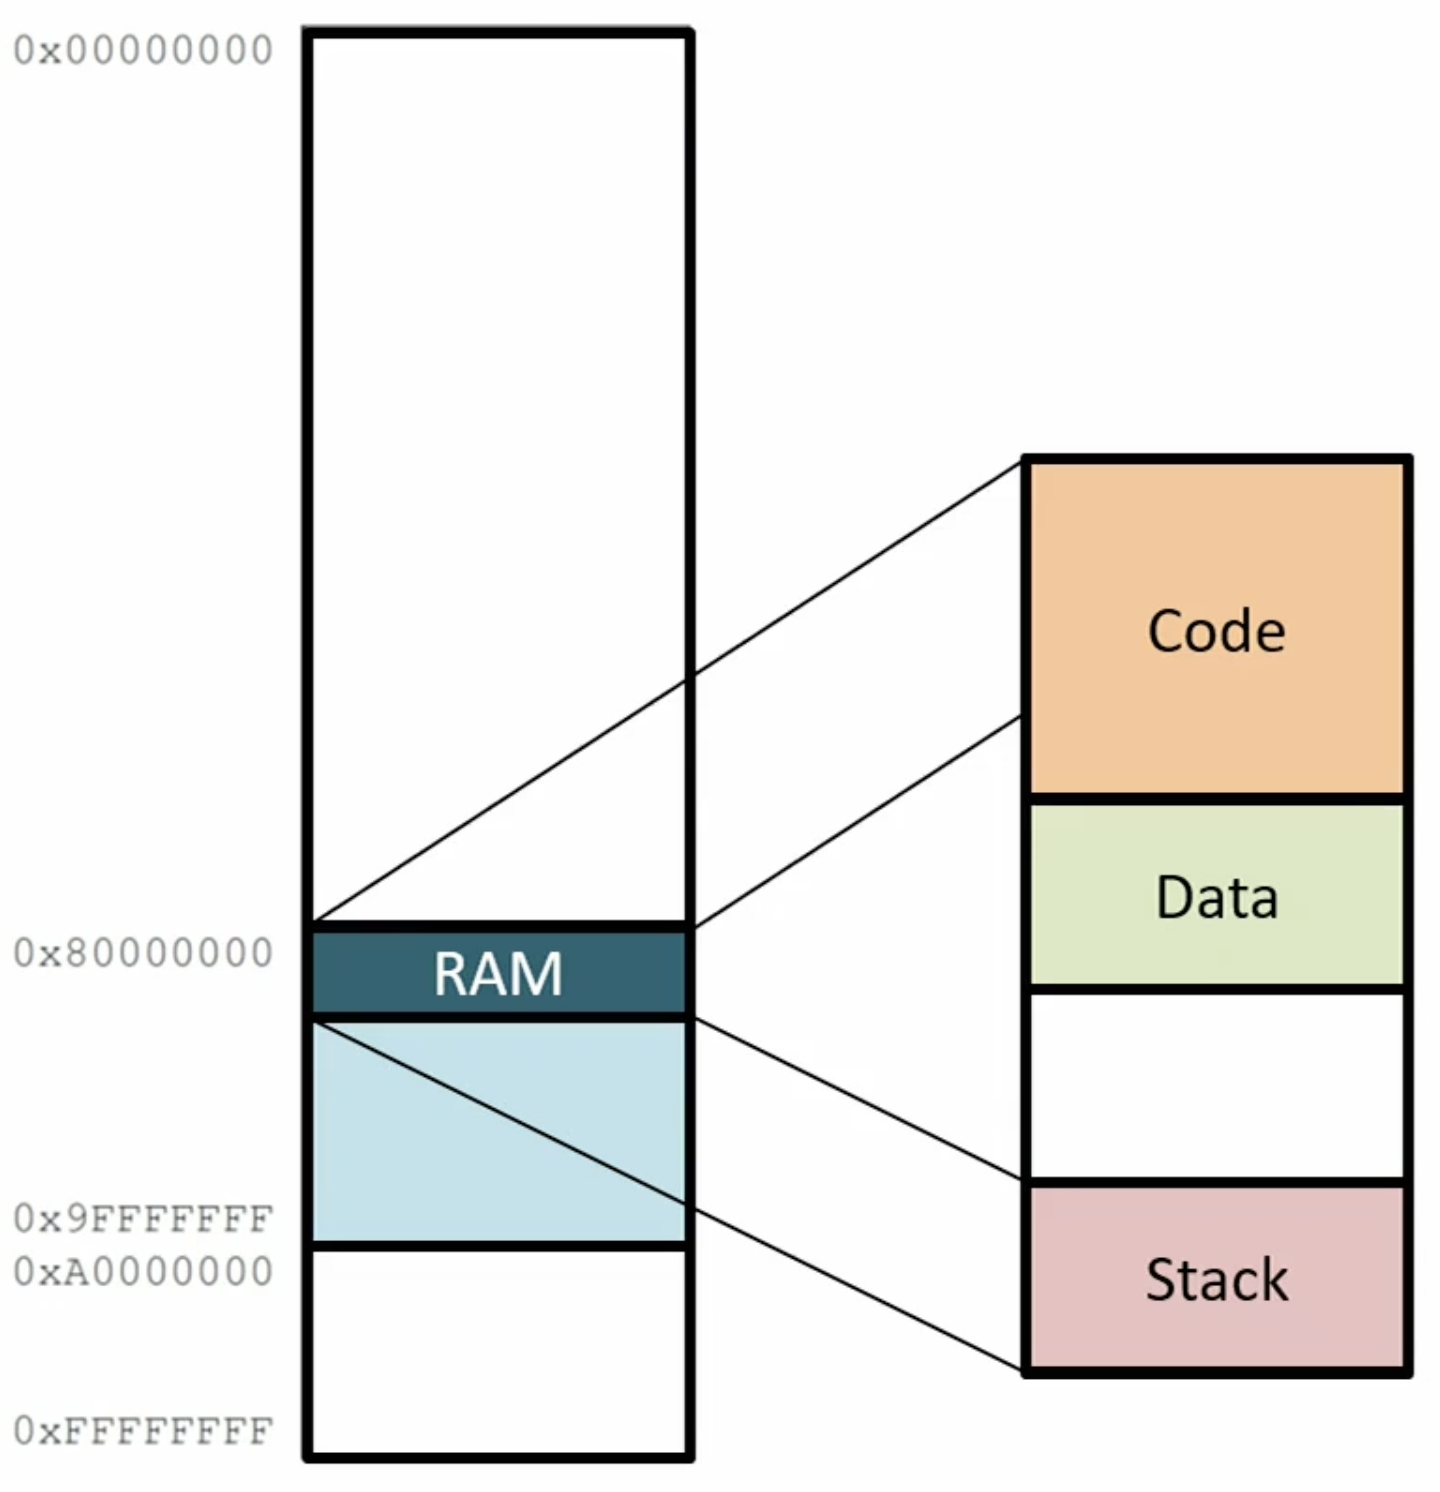
\includegraphics[width=0.35\textwidth]{chapters/chapter2b/images/memorymap.png}
\end{center}
\subsection{Connecting CPU and Memory}
\begin{center}
    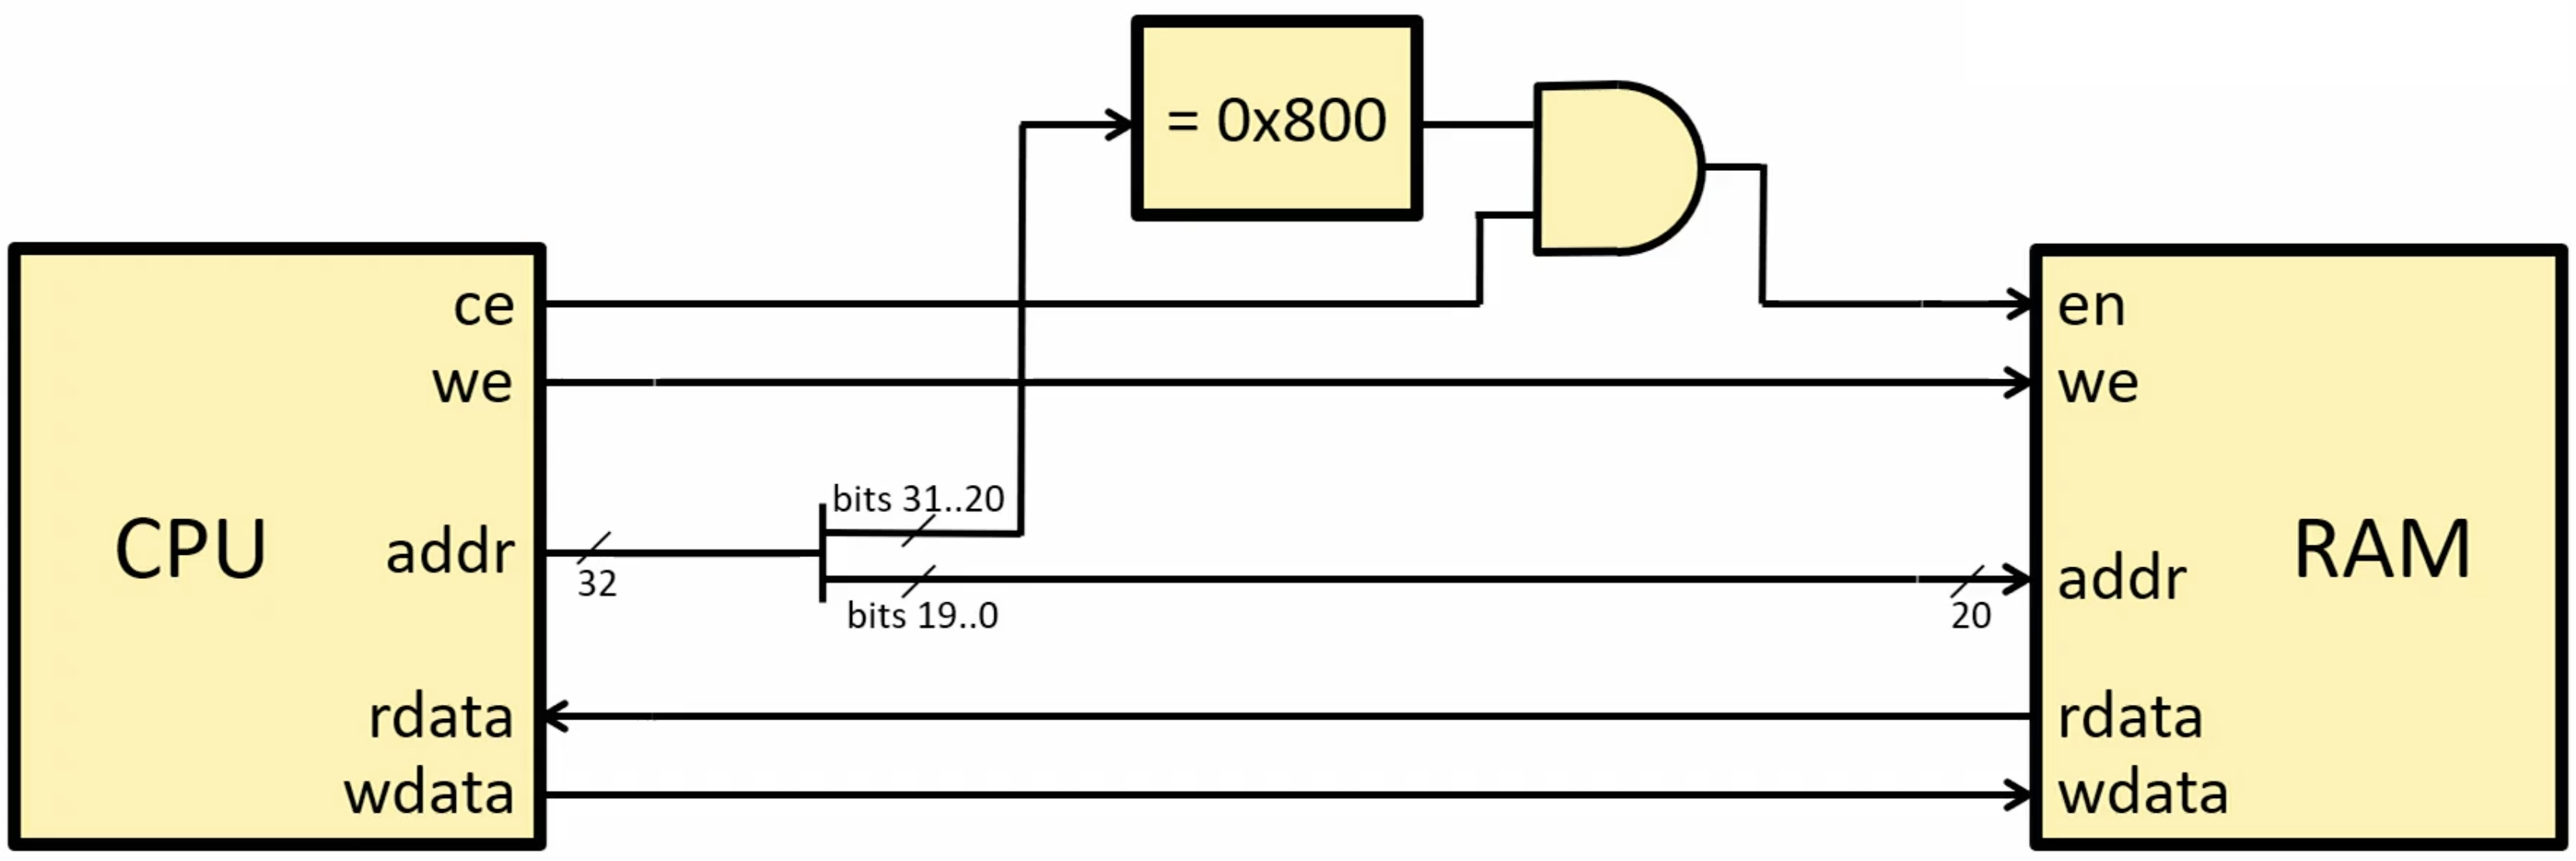
\includegraphics[width=0.65\textwidth]{chapters/chapter2b/images/cpu_memorymap.png}
\end{center}

\textbf{Address Mapping:} The upper segment of the address (bits 31..20) is compared with the hexadecimal value \texttt{0x800} to determine whether the target memory location resides within the RAM range. If the comparison (XNOR gate) yields a match, the \texttt{en} (enable) signal for the RAM is activated, allowing the subsequent read or write operation. \\
\vspace{5px}
\textbf{Control Signals:} 
Two primary control signals are involved in coordinating memory operations:
\begin{itemize}
    \item[-] \texttt{ce} (chip enable): Indicates whether the CPU is ready to perform an operation (read or write) on a specific memory chip.
    \item[-] \texttt{we} (write enable): Indicates whether the operation is a write operation, allowing data to be written into RAM.
\end{itemize}

The lower segment of the address (bits 19..0) is passed directly to the RAM as the 20-bit address input, specifying the exact memory location within the enabled RAM region. \\
\vspace{5px}
This mapping allows the CPU to access specific regions of RAM by comparing higher address bits with predefined values and appropriately enabling or disabling memory segments.
\newpage
\section{Input/Output (I/O) Devices}    
Input/Output (I/O) devices serve as crucial interfaces for various types of communication between a computer system and the external environment. 
I/O device data rates vary widely based on their type and purpose. Low-bandwidth devices like keyboards and mice handle simple inputs, while modern storage and networking technologies, such as PCIe 4.0 and USB 4.0, achieve much higher data rates for demanding tasks.
\begin{center}
    \begin{tabular}{|l|l|l|}
        \hline
        \textbf{Type} & \textbf{Peripheral} & \textbf{Data Rate} \\ \hline
        Human Interaction & Keyboard & $\sim$ kbps \\ \hline
        Human Interaction & Mouse & $\sim$ kbps \\ \hline
        Generic & Serial Port (RS-232) & 115.2 kbps (max) \\ \hline
        Generic & Parallel Port (LPT) & 150 kbps \\ \hline
        Generic & USB 4.0 & 20-40 Gbps \\ \hline
        Generic & Bluetooth 5.0 & 2 Mbps \\ \hline
        Generic & PCIe 4.0 & 16 Gbps per lane \\ \hline
        Storage & SATA III (HDD/SSD) & 6.0 Gbps \\ \hline
        Storage & NVMe (PCIe 4.0) & 64 Gbps (4-lane) \\ \hline
        Networking & Ethernet (10BASE-T) & 10 Mbps \\ \hline
        Networking & 10 Gigabit Ethernet (10GBASE-T) & 10 Gbps \\ \hline
        Networking & Wi-Fi 6 (802.11ax) & Up to 9.6 Gbps \\ \hline
        Displays & VGA (analog video) & 0.6-1.5 Gbps (approx.) \\ \hline
        Displays & HDMI 2.1 & 48 Gbps \\ \hline
        Optical Discs & CD-ROM & 150 KB/s (1x) - 7.68 MB/s (52x) \\ \hline
        Optical Discs & DVD-ROM & 1.32 MB/s (1x) - 21.1 MB/s (16x) \\ \hline
        Optical Discs & Blu-ray & 4.5 MB/s (1x) - 54 MB/s (12x) \\ \hline
    \end{tabular}
\end{center}

\subsection{Accessing I/Os: Port-Mapped I/O (PMIO)}
Port-Mapped I/O (PMIO) is a technique used to create a separate interface for Input/Output (I/O) operations, which is distinct from the memory interface. This method allows the CPU to access peripheral devices using dedicated I/O ports. In PMIO, specific control signals and new instructions are introduced to facilitate I/O operations. \\
\textit{Similar to the Memory Interface.}
\begin{center}
    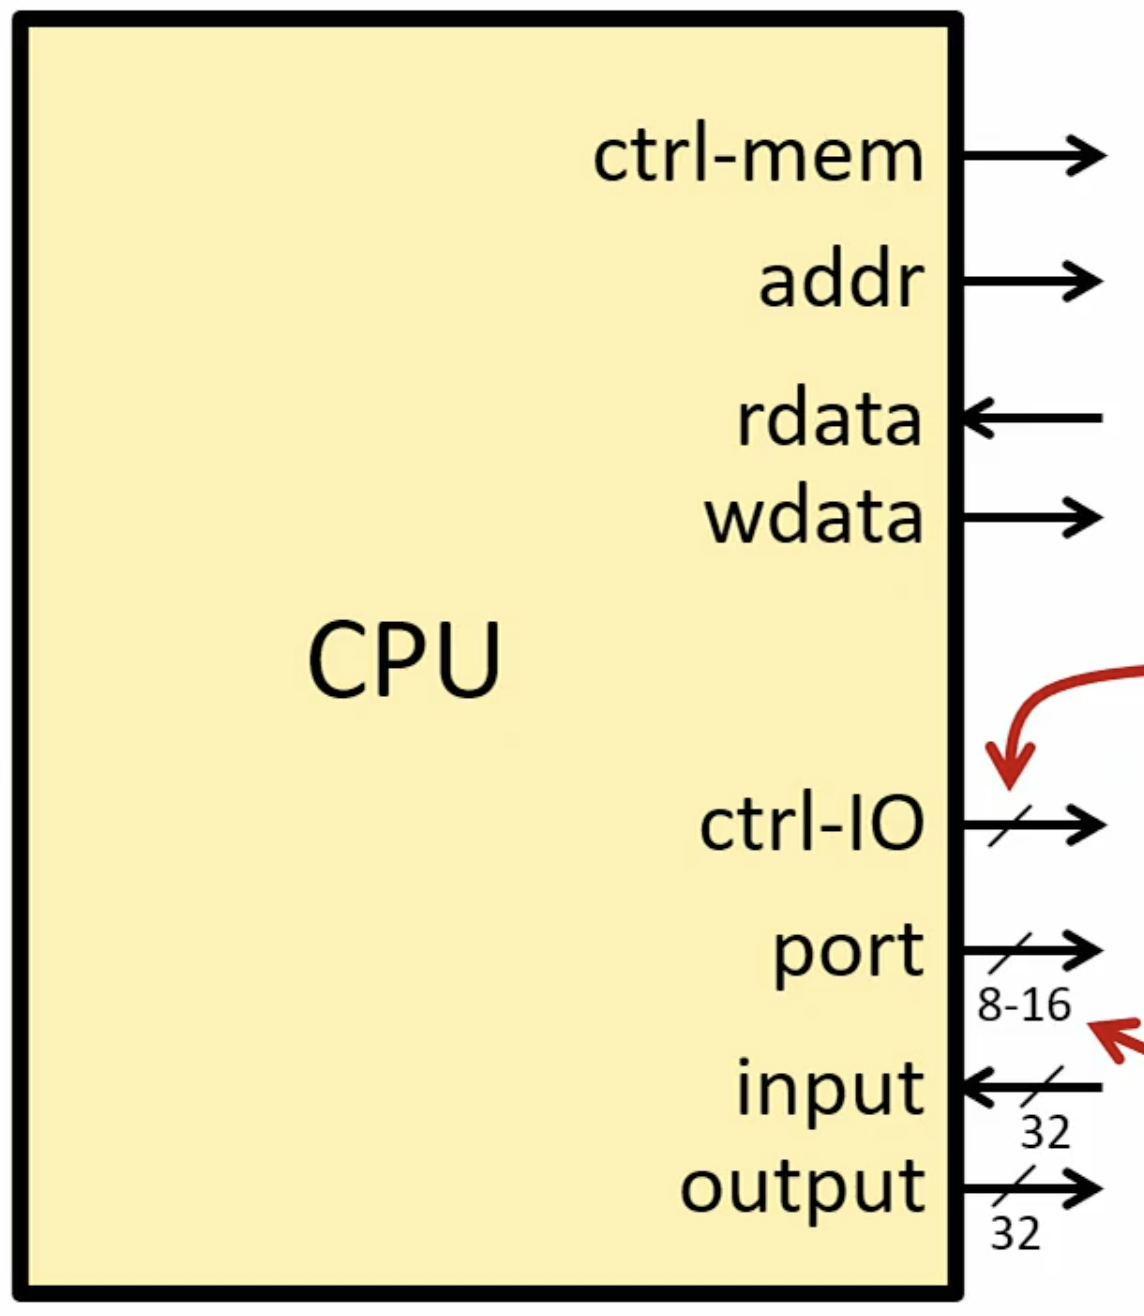
\includegraphics[width=0.25\textwidth]{chapters/chapter2b/images/io.png}
\end{center}
\begin{itemize}
    \item[-] \textbf{New Interface}: The CPU has a control interface for both memory (\texttt{ctrl-mem}) and I/O (\texttt{ctrl-IO}), along with an address bus (\texttt{addr}), read data bus (\texttt{rdata}), and write data bus (\texttt{wdata}).
    \item[-] \textbf{Port Numbering and Control Signals}: The I/O ports are addressed separately using a dedicated \texttt{port} line (typically 8-16 bits wide), and additional control signals are introduced:
    \begin{itemize}
        \item[-] \texttt{CE} (Circuit Enable): Indicates that a valid port number is provided.
        \item[-] \texttt{OE} (Output Enable): Indicates that the I/O access is an output operation.
    \end{itemize}
    \item[-] \textbf{Data Buses}: The CPU communicates with I/O devices using dedicated \texttt{input} and \texttt{output} buses, which may not necessarily be 32 bits wide due to the limited number of peripheral devices.
\end{itemize}
\subsubsection{Accessing I/Os: Memory Mapped I/O(MMIO)}
Memory-Mapped I/O is a technique that leverages the same address space for both memory and I/O operations. This allows devices to be accessed using standard memory instructions, eliminating the need for special hardware or dedicated I/O instructions. \\
\begin{minipage}[htp]{0.5\textwidth}
\textbf{Address Space Allocation}: In this configuration, specific memory addresses are allocated for different peripherals:
\begin{itemize}
\item[-] \texttt{0x1000\ 0000}: Base address for controlling LEDs.
\item[-] \texttt{0x1000\ 0010} to \texttt{0x1000\ 002F}: Address range for controlling the display.
\item[-] \texttt{0x1000\ 0030}: Base address for reading button states.
\end{itemize}
\textbf{Standard Instructions}: Since I/O devices are accessed as part of the memory space, standard load and store instructions can be used to interact with them. For example:
\begin{assembly}
# Load upper immediate to set pointer to I/Os
lui   t0, 0x10000    
# Write value in t1 to the address of LEDs    
sw    t1, 0(t0)          
# Read button states into t2
lw    t2, 0x30(t0)       
\end{assembly}
\end{minipage}
\hfill
\vline
\hfill
\begin{minipage}[htp]{0.45\textwidth}
    \begin{center}
        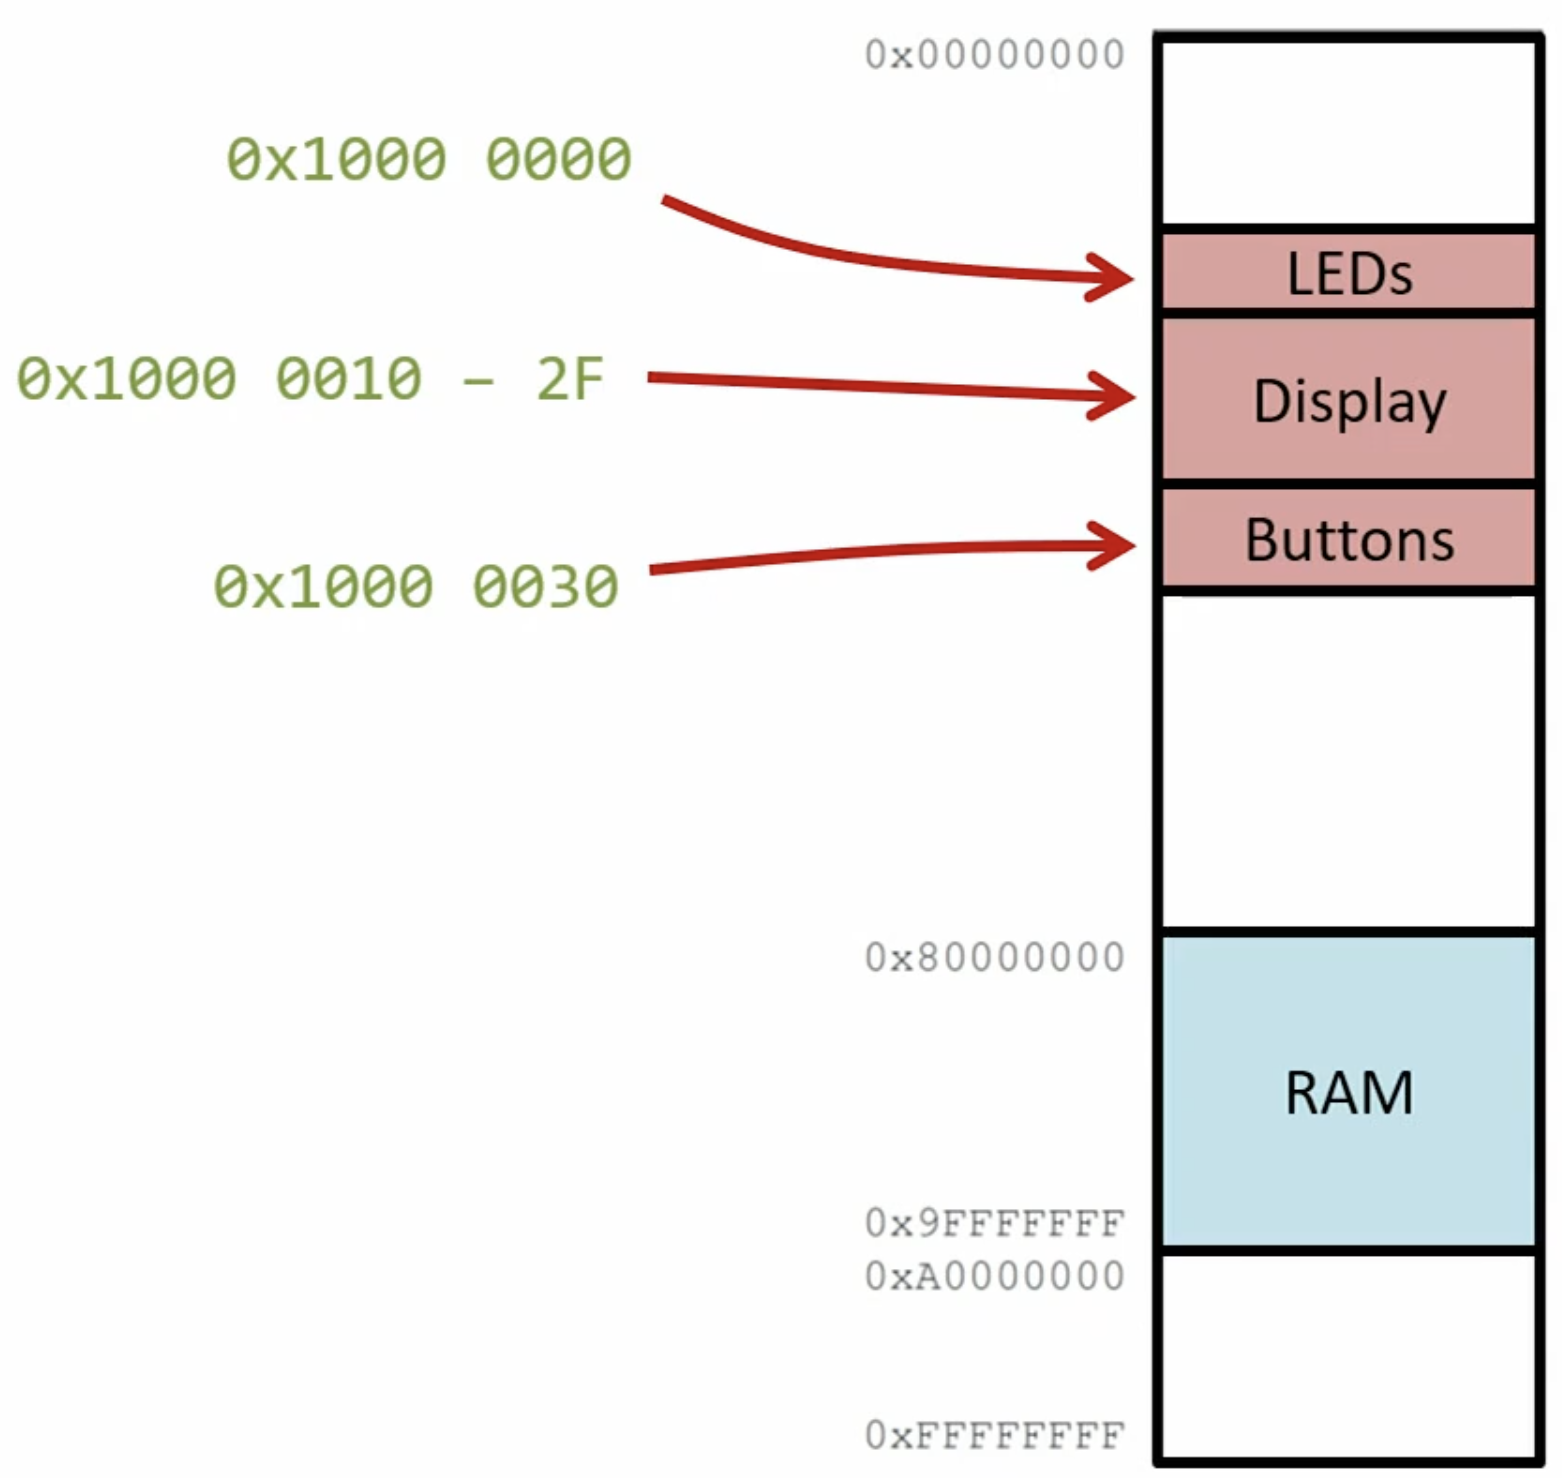
\includegraphics[width=1\textwidth]{chapters/chapter2b/images/io_memory.png}
    \end{center}
\end{minipage}\\
\vspace{5px}


\subsection{Memory Mapped I/O (MMIO)}

In computer architecture, Memory-Mapped I/O (MMIO) is a technique used to access input and output devices. Instead of using separate I/O instructions, devices are assigned specific memory addresses. The CPU interacts with these devices by reading or writing data to these memory locations as if they were normal memory addresses.

\begin{center}
    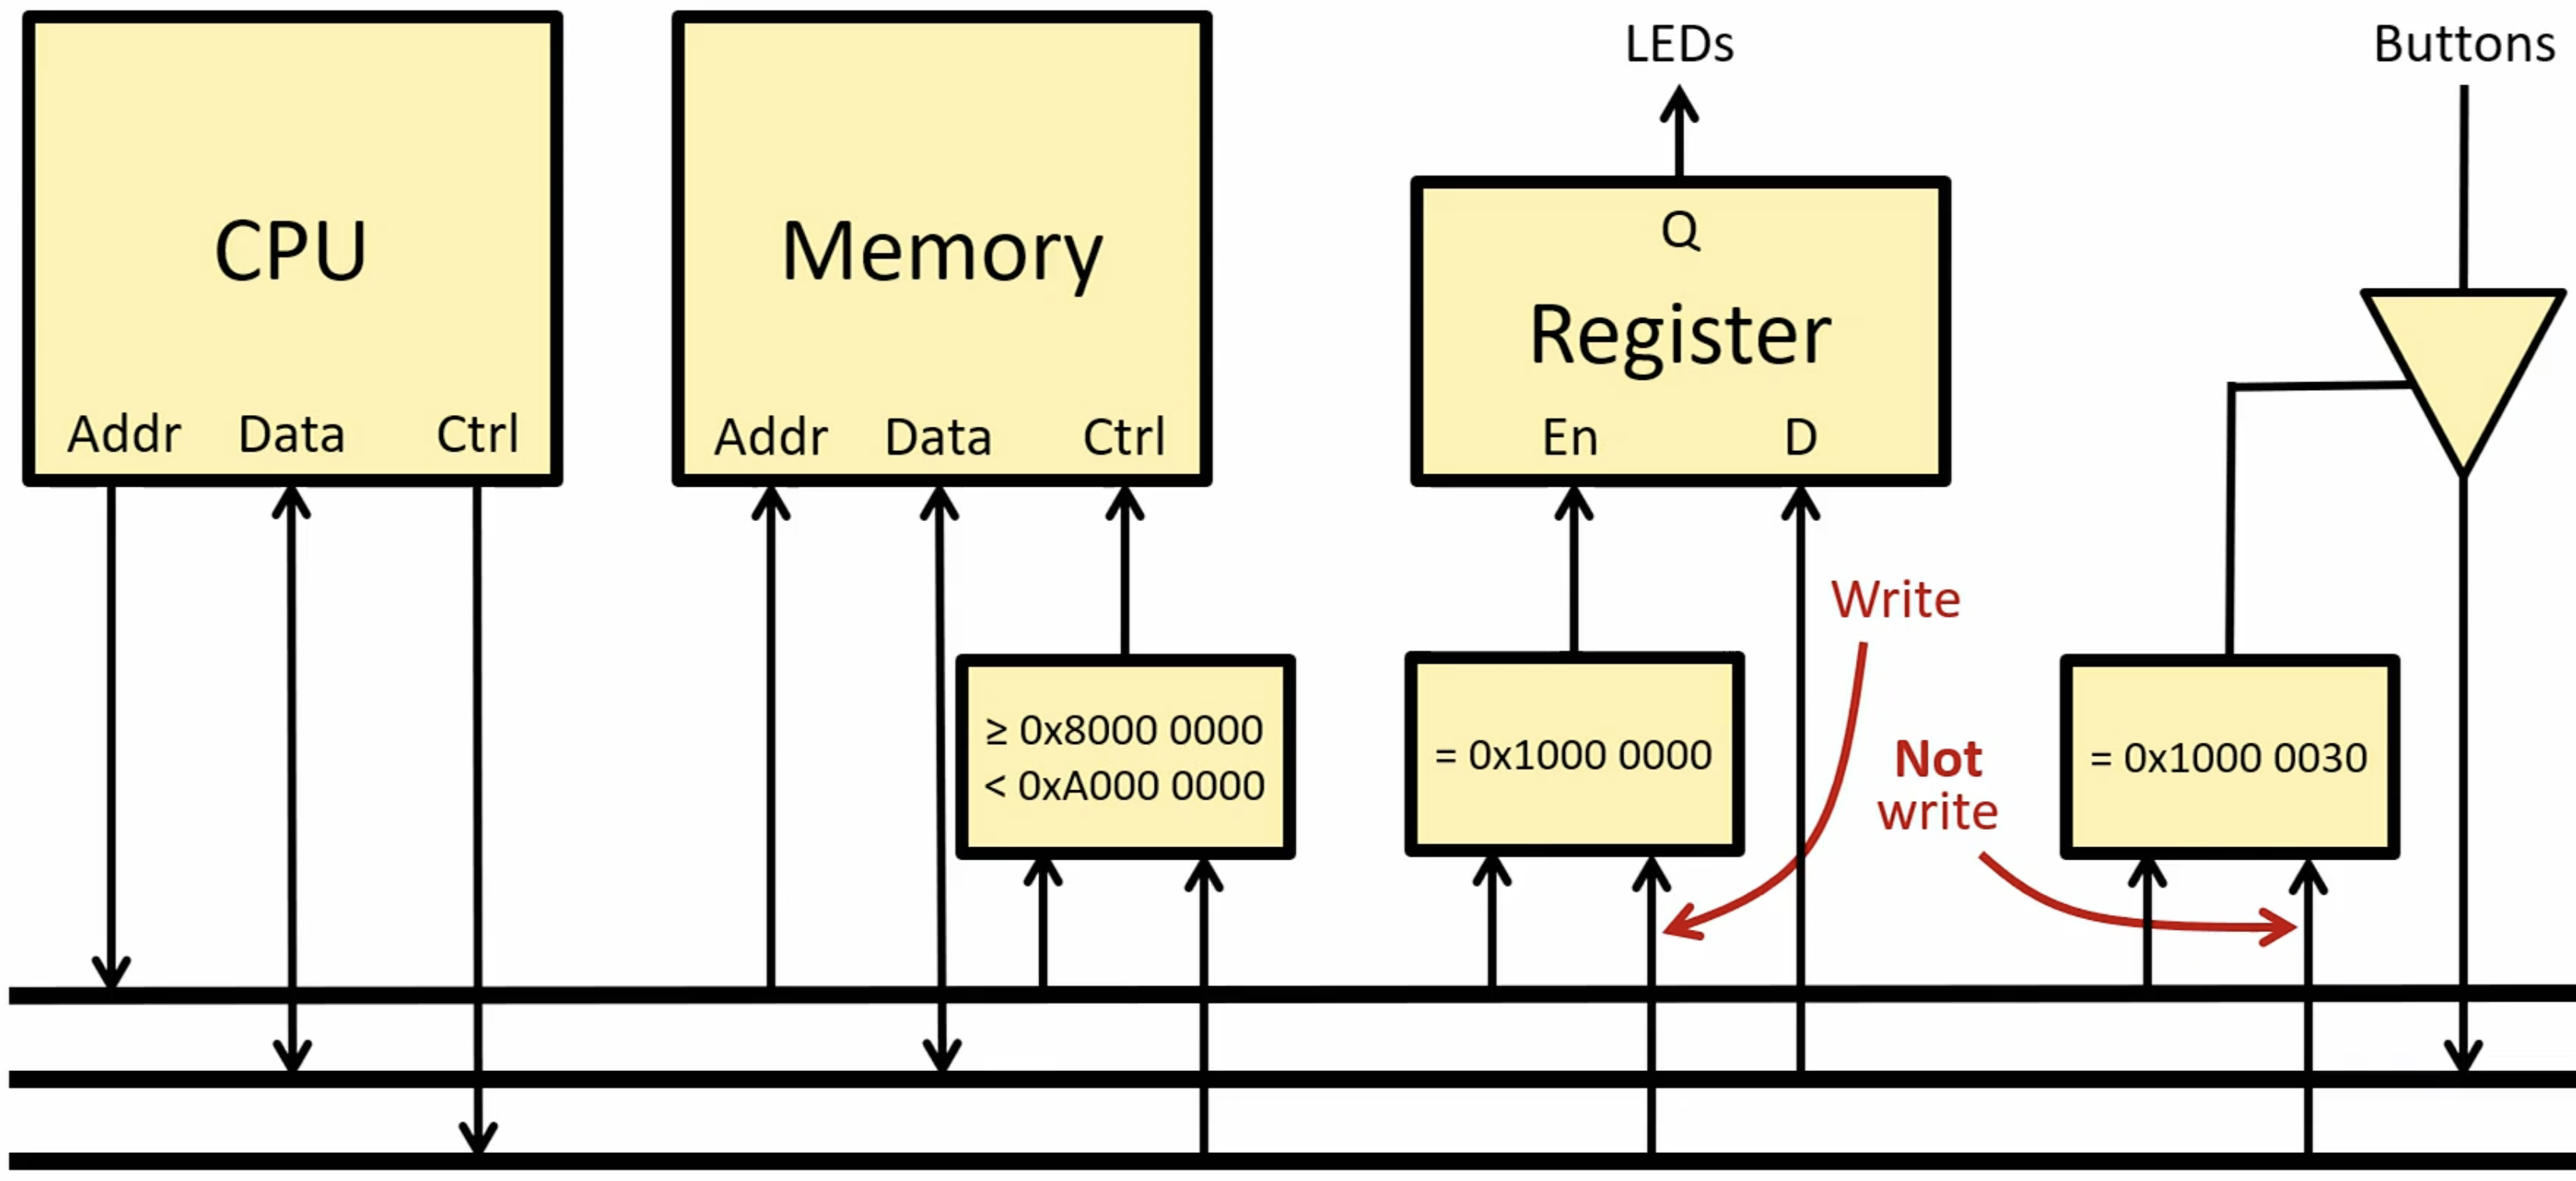
\includegraphics[width=0.65\textwidth]{chapters/chapter2b/images/complete.png}
\end{center}

\subsubsection*{Components}
\begin{itemize}
    \item[-] \textbf{CPU:} Acts as the central processing unit that interacts with memory and registers. It uses address, data, and control buses to communicate.
    \item[-] \textbf{Memory:} Represents the conventional memory address space accessible by the CPU. Specific memory ranges (e.g., between $0x8000\ 0000$ and $0xA000\ 0000$) are reserved for memory-mapped devices.
    \item[-] \textbf{Register:} The CPU communicates with the register through a dedicated memory-mapped address (e.g., $0x1000\ 0000$ for writing operations). This register drives outputs such as LEDs or accepts inputs from buttons.
\end{itemize}

\subsubsection*{Operation}
The CPU interacts with memory and I/O devices through common buses. Depending on the address, data is either directed to regular memory or to an I/O device register. When the address matches a specific register (e.g., $0x1000\ 0000$ for a write operation), the corresponding action is triggered, such as updating an LED state. In contrast, accessing $0x1000\ 0030$ might perform a read operation, retrieving button states.
\section{Example - A/D Converter}
This example describes an Analog-to-Digital (A/D) Converter or (ADC) and its associated signals. The A/D Converter converts an analog input signal into a digital representation. The conversion process and signal behaviors are described below.
\subsubsection*{Signals}
\begin{itemize}
    \item[-] \texttt{\textbf{Start (START):}} This input signal, when active a new conversion begins.
    \item[-] \texttt{\textbf{Data Valid (/DV):}} This output signal indicates the validity of the data. When active, the output data bits (\texttt{D7-D0}) contain the converted digital value and are Valid.
    \item[-] \texttt{\textbf{Data (D7-D0):}} The output data bits representing the last conversion result in digital form.
\end{itemize}

\subsection{Bus Interface}
The A/D Converter interacts with an 8-bit processor using a simple bus interface. This bus interface allows data exchange and control signals to flow between the A/D Converter and the processor. The following signals are used:

\begin{itemize}
    \item[-] \texttt{\textbf{Address (A23--A0):}} Output - Serves as the address bus to select a specific device or memory location.
    \item[-] \texttt{\textbf{Data (D7--D0):}} Bi-directional - Represents the data bus used for data exchange between the processor and the A/D Converter.
    \item[-] \texttt{\textbf{Address Strobe (/AS):}} Output - Indicates the presence of a \textbf{valid} address on the address bus during a memory access cycle.
    \item[-] \texttt{\textbf{Read/Write (R//W):}} Output - Determines the direction of the data flow (read from or write to the A/D Converter).
    \item[-] \texttt{\textbf{Data Acknowledge (/DTACK):}} Input - Signals the completion of a memory access by the A/D Converter when activated, indicating that the data is ready or has been latched.
\end{itemize}

The bus interface provides a simple mechanism for connecting the A/D Converter to the system bus, allowing the processor to initiate conversions and read the results.

\subsection{Memory Mapping}
The A/D Converter is connected to the processor using a memory-mapped interface. Specific memory addresses are reserved for starting conversions, reading the data valid signal, and accessing the conversion result. The following address mapping is used:
\begin{itemize}
    \item[-] \texttt{\textbf{0xFFFFF0:}} Any access (read or write) to this address initiates a new conversion by the A/D Converter.
    \item[-] \texttt{\textbf{0xFFFFF4:}} The processor reads the data valid signal from this address. Bit 0 of this location indicates whether the conversion result is ready.
    \item[-] \texttt{\textbf{0xFFFFF8:}} The processor reads the conversion result from this address. The value stored here represents the digital output of the A/D Converter.
\end{itemize}

This memory-mapped interface simplifies the interaction between the processor and the A/D Converter by using standard read and write instructions to control the conversion process and retrieve the results.
\newpage \subsection{Assembling everything}
\textit{To get to this point, it is highly advised to first draw a timing diagram of the expected signals, and then start drawing connections, also, be careful, the notation "/AS" for example, means that the signal is active low.}
\begin{center}
    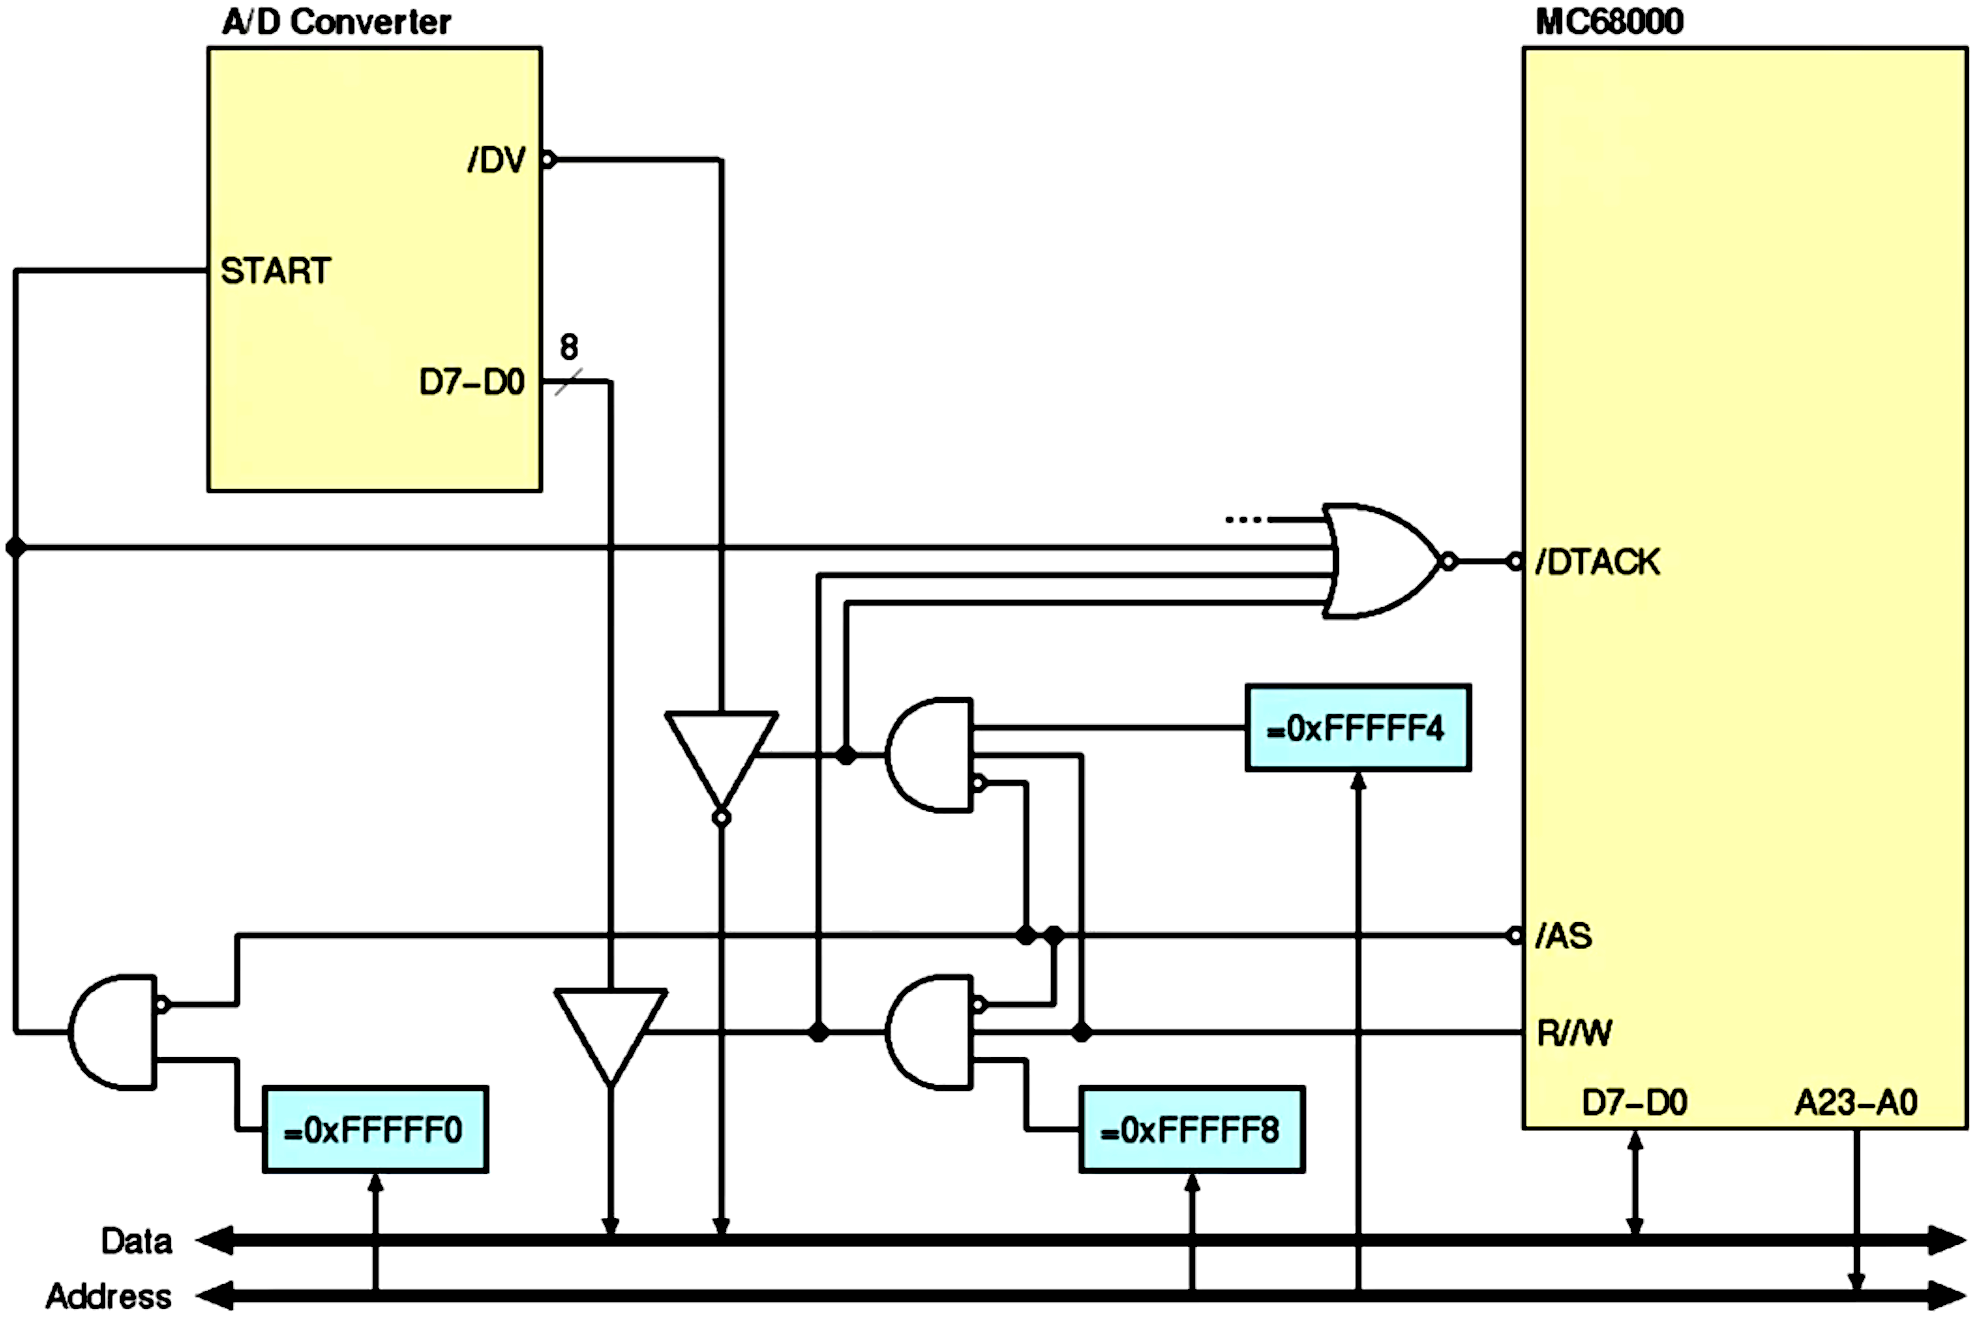
\includegraphics[width=0.55\textwidth]{chapters/chapter2b/images/adc.png}
\end{center}
\subsubsection{Software Implementation}
\begin{center}
\begin{assembly}
.section .data
START_ADDR:      .word 0xFFFFF0     # Address to initiate conversion
DATA_VALID_ADDR: .word 0xFFFFF4     # Address to check if data is valid
RESULT_ADDR:     .word 0xFFFFF8     # Address to read conversion result

.section .text
.globl _start

# Start of the main program
_start:
    # Initiate A/D Conversion
    lui t0, %hi(START_ADDR)       # Load upper 20 bits of START_ADDR
    lw t1, %lo(START_ADDR)(t0)    # Load lower 12 bits into t1
    # Write zero to start the conversion (writing to address 0xFFFFF0)
    sw zero, 0(t1)               

wait_for_data:
    # Check if the data is valid
    lui t0, %hi(DATA_VALID_ADDR)  # Load upper 20 bits of DATA_VALID_ADDR
    lw t1, %lo(DATA_VALID_ADDR)(t0) # Load lower 12 bits into t1
    lw t2, 0(t1)                  # Load the data valid status into t2
    andi t2, t2, 0x1              # Mask bit 0 (check if data is ready)
    beq t2, zero, wait_for_data   # If bit 0 is zero, data is not valid, wait

    # Read the conversion result
    lui t0, %hi(RESULT_ADDR)      # Load upper 20 bits of RESULT_ADDR
    lw t1, %lo(RESULT_ADDR)(t0)   # Load lower 12 bits into t1
    lw t3, 0(t1)                  # Read conversion result into t3

    # End of program (infinite loop)
end:
    j end                         # Loop indefinitely        
\end{assembly}
\end{center}
\newpage 
\section{What do these tri-state buffers do?}
\textit{Tri-state buffers are crucial components used to control data flow on a bus. They can exist in one of three states: high impedance (effectively disconnected), logic high, or logic low.}
\\
\textit{If not controlled properly, a tri-state buffer can cause bus contention, where multiple devices attempt to drive the bus simultaneously, leading to data corruption or damage.}

\begin{center} 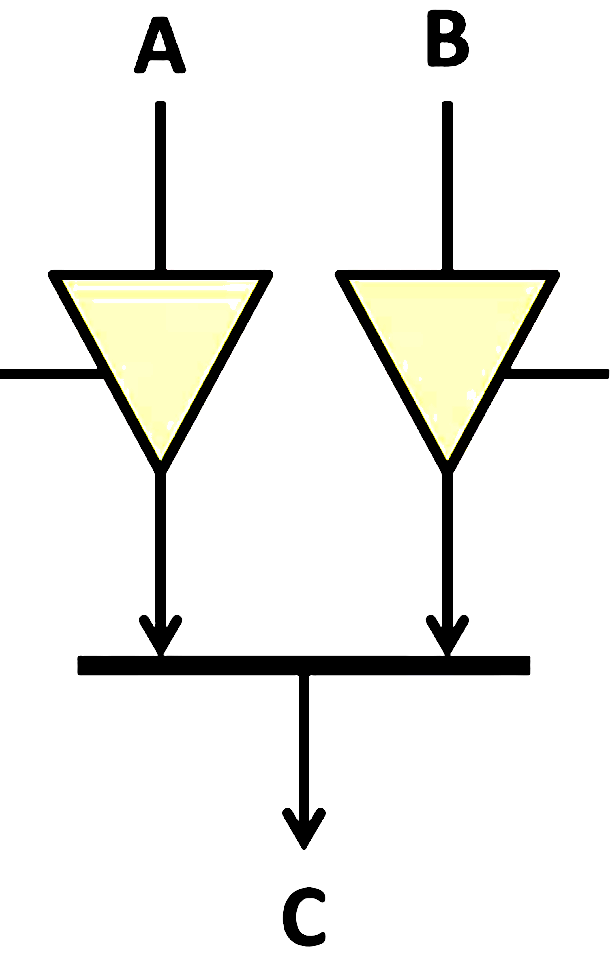
\includegraphics[width=0.20\textwidth]{chapters/chapter2b/images/tris1.png} \end{center}

In essence, a tri-state buffer acts like a decentralized multiplexer, functioning similarly to a multiplexer with a select line to manage data transmission.

\begin{center} 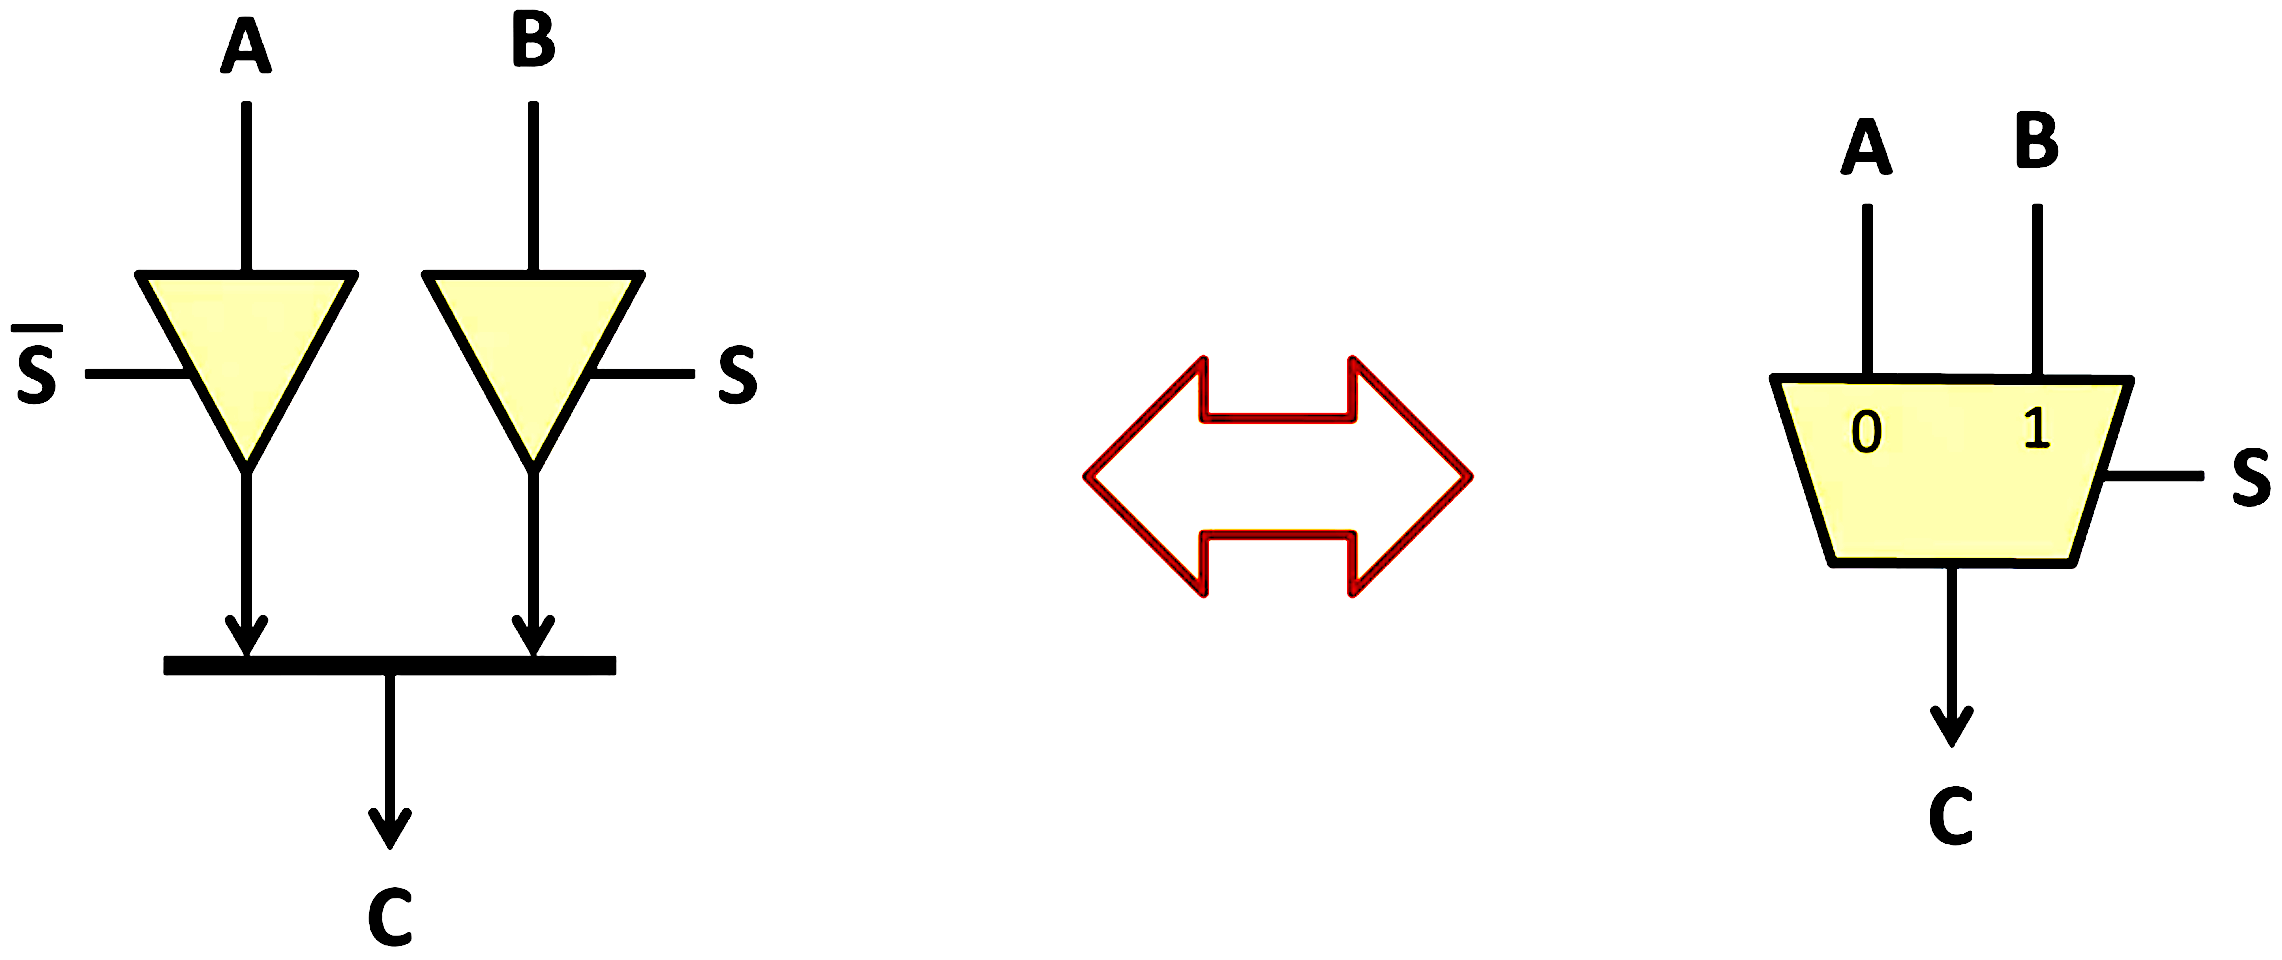
\includegraphics[width=0.75\textwidth]{chapters/chapter2b/images/tris2.png} \end{center}
\newpage
\subsection{A Classic UART}

\textbf{UART (Universal Asynchronous Receiver-Transmitter)} is one of the simplest and most common communication peripherals, typically used to connect terminals to embedded devices. 

Our UART employs a simple programmed I/O interface, consisting of four key registers:

\begin{itemize}
    \item[-] \textbf{Control register}: Configures the UART. Bit 7 must be set to 1 to enable the UART, while bits 2 to 0 determine the communication speed (e.g., \texttt{0b001} for 9600 baud).
    \item[-] \textbf{Status register}: Provides the current status of the UART. Bit 1 indicates if data is available, and bit 0 signals if the UART is ready to transmit data.
    \item[-] \textbf{Data input register}: Holds the received data available to the processor.
    \item[-] \textbf{Data output register}: Contains data placed by the processor for transmission.
\end{itemize}

\begin{assembly}
# Constants
UART_CTRL_ADDR      = 0x10000000  # UART control register address
UART_ENABLE_BIT     = 0x80        # Enable bit (bit 7)
UART_SPEED_9600     = 0x01        # Speed setting for 9600 baud (4 bits, [3:0])
UART_STATUS_ADDR    = 0x10000004  # UART status register address
TX_READY_BIT        = 0x01        # Transmitter ready bit (bit 0)
UART_DATAIN_ADDR    = 0x10000008  # UART data input (receive) register address
UART_DATAOUT_ADDR   = 0x10000008  # UART data output (send) register address

# Send a string using UART
send_string:
    li t0, UART_CTRL_ADDR         # Load UART control register address into t0
    li t1, UART_STATUS_ADDR       # Load UART status register address into t1
    li t2, UART_DATAOUT_ADDR      # Load UART data output register address into t2
    li t3, UART_ENABLE_BIT        # Load enable bit (0x80) into t3
    li t4, UART_SPEED_9600        # Load speed setting (0x01) into t4
    or t3, t3, t4                 # Combine enable and speed bits into t3
    sw t3, 0(t0)                  # Configure UART by storing combined value into control register

next_char:
    lb t5, 0(a0)                  # Load the current byte of the string into t5
    beqz t5, finish               # If the byte is zero (null terminator), jump to finish

check_tx_ready:
    lw t6, 0(t1)                  # Load the value of the UART status register into t6
    andi t6, t6, TX_READY_BIT     # Check if the TX ready bit is set
    beqz t6, check_tx_ready       # If not ready, loop back to check again

    sw t5, 4(t2)                  # Store the character in UART data register
    addi a0, a0, 1                # Move to the next character in the string
    j next_char                   # Jump to send the next character

finish:
    ret                           # Return from function
\end{assembly}

